\chapter{Methodology}
This chapter will focus on the research methodology and design.
Before going into the research design, the reasoning for the use of qualitative research model will be discussed.
%Secondly, the research design will be discussed of which qualitative research method is used in the form of multiple case study which will be explored to get the required information for this study. 
Then the case criteria selection and the data collection methods will be given.
%------------------------
%Waarden ophalen uit database

When doing research, two basic methods can be distinguished, qualitative and quantitative~\citep{Saunders:2009wn}.
When researchers try to discover causal links between two or more subjects quantitative research is deemed most appropriate~\citep{van2008management}.
In this thesis the data will be analysed using what~\citep{Saunders:2009wn} refers to as `non numeric' data, hence this research study is qualitative in nature.
To determine motivations, perceptions or beliefs of a certain phenomenon~\citep{van2008management,Eisenhardt:1989ww} qualitative research is considered most appropriate.
The study will be done in a mono-method capacity, hence no quantitative data will be used in this research~\citep{Saunders:2009wn}.
The qualitative case study methodology provides tools for researchers to study complex phenomena within their contexts~\citep{Baxter:2008vu,Ryan:2003hn}.\\
%Amongst all philosophical assumptions reviewed, the interpretive paradigm has been identified as the most appropriate framework to use for this study~\cite{Yin:2009vh}. 
\section{Multiple Case Study Research Design}

The research design explains the structure of research. 
In fact, it explains how research is conducted and how the subsequent data is analysed~\citep{van2008management}.
To collect the (qualitative) data for this study the method of the multiple case study has been selected.\\
According to~\cite{Yin:2009vh} case studies differentiate from other types of studies in that an attempt is made to examine a contemporary phenomenon within a real-life context. 
The technique of case studies is mostly employed when there are no clear boundaries between that particular phenomenon and it’s context~\citep{Yin:2009vh,Marshall:1996wc}.
Clearly the effects of the WTO on \gls{IB} and the firms within the \gls{IB} environment are a real-life current phenomenon. 

The multiple case study differs from the single case study~\citep{van2008management,Yin:2009vh}.
The single case study is often used when dealing with an exceptional situation, where the multiple case study deals more than one case, having the benefit replication across cases~\citep{Saunders:2009wn}.
The (qualitative) multiple case study is an approach to research that facilitates exploration of a phenomenon within its context using a variety of data sources~\citep{Baxter:2008vu}.
This ensures that the issue is not explored through one lens, but rather a variety of lenses, which allows for multiple facets of the phenomenon to be revealed and understood~\citep{Baxter:2008vu}.
This is an approach to research that facilitates exploration of a phenomenon within its context using a variety of data sources~\citep{Baxter:2008vu}.\\
The advantage of this method is, it assures a richness of content, as~\cite{Eisenhardt:1989ww} explains and can lead to novel, testable and rich information.\\
%The \mcs approach can lead to novel, testable and rich information.
However, the disadvantage of this method is that the results are not statistically generalisable~\citep{Yin:1981wc}.  
By investigating a phenomenon at one particular location, cross-sectionally and with only few organisations within the sample as units of analysis, this would result in lower generalisability~\citep{Klossek:2012wc}. 
The results are only valid in a specific setting for specific type of organisations~\citep{Deng:2007tr}.
This research method aims to describe, rank and explore data with the aim of generating working propositions or illustrating an existing theory~\citep{Eisenhardt:1989ww,Yin:1981wc}.\\
The multiple case study can been seen as the ideal method of collecting data and or information for this research question~\citep{Yin:2009vh}.
In this thesis, two different regions in the world, based on the economic development of those regions (\glspl{EE} vs. \glspl{AE} see also Appendix~\ref{app:AEnEE}), are investigated.
Next to the two (economic) regions, two industries within these economic regions, the \pharma and ICT services industries (that are governed by WTO \rr) are analysed. 
The rationale behind the choice of these two industries and specific companies is explained in Section~\ref{sec:rational}.
%By investigating a certain phenomenon at only one particular location, cross-sectionally and with only a few organisations within the sample as units of analysis, this could result in lower generalisability (Klossek et al, 2012; Deng, 2007). 
%On has to keep track of the fact that the results are only valid in a combination of specific settings and organisations.

This research method aims to discover not as much explanatory, but moreover exploratory findings~\cite{Yin:1981wc} on the effects of the WTO \rr.
The `why' question for~\mcs is associated with explanatory research questions~\cite{Yin:2009vh}, this thesis does not seek to answer those.
Here the question is whether the WTO effects some companies in certain countries or regions differently. 
Hence the research question is an exploratory one~\citep{Yin:2009vh,Miles:1994wi}.\\
In this research, the propositions were developed prior to carrying out the case study research. 
This is in line with~\citep{Yin:2009vh,Hyde:2000hf} (multiple) case study approach.

\section{Case Criteria and Selection}

The next step is to identify and select the cases that will be used. 
As mentioned by~\cite{Pettigrew:1990}, the number of cases that are studied is usually limited, therefore it is a good approach to select cases that signify correctly the differences at hand.
%The research approach aims to obtain in this way exploratory, as well as explanatory findings. The exploratory element would refer to how some variables might influence the degree of knowledge sharing; the explanatory element would provide insight in how some variables should be adjusted in order to enhance inter- business unit knowledge sharing for multi-domestic MNEs (Yin, 2012).
In the selection process certain boundaries have been set to ensure a comprehensive selection can be made.
The selection of the firms will be made on a number differentiating levels.
The first differentiating level will be economic region.
The second will be on type of industry.

\subsection{Economic Region Selection}

The aim of this study is to compare the effects of the \gls{WTO} decisions on  \gls{EE} and \gls{AE} firms.
Hence the cases will be selected from \gls{EE} and \gls{AE} firms.
The terms \gls{EE} and \gls{AE} have been defined in Appendix~\ref{app:AEnEE} and the specific economic regions or countries associated with the \gls{EE} and \gls{AE} are also listed in this Appendix.

The region that has been selected as \gls{AE} is the European Union. 
To create a larger potential group of firms (MNEs) the \gls{EU} has been selected as opposed to a single european country.
As this thesis is written in a European environment is seems only logical to choose Europe as the \gls{AE}.

As for a \gls{EE} a number of choices as possible.
The obvious choice in this case would be China.
There is already a lot of research being done on China and Chinese MNEs~\citep{Deng:2012to,Alon:2011um}.
However India does make for a very interesting candidate.
The exposure India as a country and economic power receives, might be less than China.
The Economist does have a separate section on China but does not have one on India for example.
But India is a more than capable alternative.
India is among the largest economies of the world, measured by \gls{GDP}.
In 2012 the \gls{GDP} of India ranked 4th (with the EU, US and China making up the top three)~\citep{CIA:2013}.
India has a have a well established services sector contributing over 50\% to \gls{GDP}~\citep{Government-of-India:2012}.
The Indian IT services industry has a global reach, where the Chinese is more domestic oriented~\cite{Raman:2011jm}.
India might be less known as a manufacturer compared to China~\citep{Daily-Mail:2010}, it does have a lot of potential~\citep{Dhawan:2012ws}.\\
China and India are both capable EE and are among the top four economies in the world.
The global character of both the Indian services and the Indian \manu industries make for a very interesting \gls{EE}.
Therefor India has dully been selected.

%Viewed from a global point of view, the influence of the \wto~spans the entire globe. 
%This playing field is than decided into two economic blocks: \gls{EE} and \gls{DE}. 
%As these two blocks span a great number of countries and continents, India (an \gls{EE}) and the \gls{EU} have been chosen to represent the two economic blocks. 
%Both India and the EU have an equally long standing relation with the \wto~and have been active in the various life cycles of the \wto~for a great number of years.\\
%The next level of distinction that can be determined is the industry level. 
%Within both the EE and DE one can find different industry types.

\subsection{Industry Selection}\label{sec:rational}

In~\cite{Porter:1980to} already identified the importance of industries in the search for~\ca. 
The industry types have to be existent in sufficient quantities in both economic blocks.
For a good comparison looking at different industry types seems logical. \\
\cite{Fisher:1939} defined three industry sectors; the Primary, Secondary and Tertiary sectors.
The primary sector consists mainly of raw material sourcing companies, the secondary sector has to do with manufacturing and the tertiary sector consists of services firms.
For the purpose of this research we will focus on firms from the secondary and tertiary sectors~\citep{Fisher:1939}.
%To be able to make an accurate comparison, firms that will be chosen have to be present in both industries and in both the European Union and India.


\subsubsection{Manufacturing Industry} 

%For the manufacturing industry, the pharmaceutical industry has been selected.
To be able to come to a comprehensive comparison, the sectors under investigation are to be both present in the \gls{EE} and the \gls{AE} alike. 
This is the case for the \pharma industry in both \gls{EU} and in India.\\
The pharmaceutical has been long present in the EU\@. 
Especially Germany, Switzerland and Brittain have a history (dating back to the 18th century) in the pharmaceutical business~\citep{Walsh:2010,Liebenau:1984wb}.
Although not as old as the European history, India does have a history in the \pharma industry~\citep{Mazumdar:2012tx}. 

Not of primary concern, but still useful, the \pharma sector has decent size firms in both \gls{EU} and India.
Hence the amount of information is expected to be sufficiently available on companies in these regions and sectors.


\subsubsection{Services Industry} 

As a service the~\gls{IT} services industry is very much on the move and an example of the globalisation of the workplace~\citep{Reuters:2012}. 
Development centres are being set up all over the world~\citep{Reuters:2012,India-Times:2008}. 
As for the services industry, India is well known for their ICT services industry. 
One might argue that India has a leading role in the~\gls{IT} services and~\gls{BPO} practices~\citep{The-Hindu:2011}. 
The I(C)T services industry is one of the largest Industries of India. 
It accounts for 41.7\% of the total services export~\citep{Government-of-India:2012}.
One can conclude the~\gls{IT} services industry is well established in India and could be solid choice as a services industry example.

In Europe and the~\gls{EU} the~\gls{IT} services firms do not see the same amount of growth as the Indian industry however there are still some large companies active~\citep{Deloitte:2010}. 
Much of the~\gls{IT} services is about outsourcing~\gls{IT} work\footnote{More on the working practices of the~\gls{IT} services industry can be found in~\ref{sec:sevicesFirms}}.
For this reason all~\gls{IT} services firms have a global presence and a lot of the actual (coding) work is done in low-wage countries (like India). 
Notwithstanding this globalisation aspect, Europe still boasts a healthy number of~\gls{IT} services companies~\citep{Computer-Weekly:2011} that can be analysed in this thesis.
Overall the~\gls{IT} services industry in Europe is a healthy one to serve as a services industry example.

%Distance is not a factor when it comes to delivering a ~\gls{IT} solution.
%One can send an application across half the world in a matter of seconds. 
Both the~\gls{IT} services and \pharma industries seem interesting industries to focus on, with regard to the services they provide and in the light of the division in industries as defined by~\citep{Fisher:1939}.


\subsubsection{Firms}

Finally with the industries defined, firms can be selected. 
To be able to find as much information as possible multinational \pharma companies have been selected from both the European and Indian markets.\\
The Indian \pharma companies are Ranbaxy and Cipla.\\ %(possibly Dr Reddy's).
The choice of these two companies is base on the size, they are among the largest in India and have a decent amount of growth (see Figure~\ref{fig:IndiaPharma}).

\begin{figure}[htbp] 
	\centering
	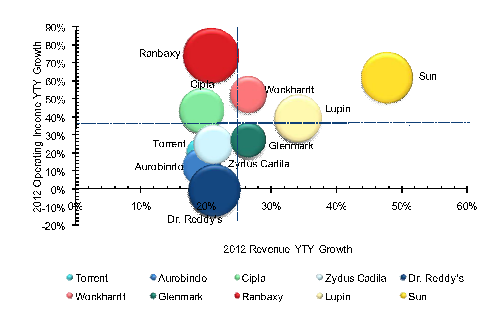
\includegraphics[width=0.8\textwidth]{IndiaPharma.eps}
 	\caption[Competitive Landscape of the Top 10 Pharmaceutical Companies in India]{Competitive Landscape of the Top 10 Pharmaceutical Companies in India, 2012. source:~\citep{Research-and-Markets:2013}}\label{fig:IndiaPharma}
\end{figure}

Many European \pharma companies have merged with or have been purchased by US firms. 
The focus will be on firms that have no original ties with the US through mergers.
This limitation has been considered to be able to include only firms into the research, that have the most European pedigree as possible.
As counterparts for the Indian firms we will choose Novartis and GSK as the European contenders.
Both the European firms are top 20 of \pharma~companies\footnote{\url{http://www.contractpharma.com/issues/2013-07/view_features/top-20-pharma-report-/}} in the world.\\
As for the ICT services firms in India there is a lot of choice. 
Here we opt for pure Indian companies not only have their operations in India, but the management and ownership are Indian as well.
For these reasons, Infosys and WiPro have been selected. 
%(TCS) is used as a backup company as they are not purely a ICT company.
Both companies are among the largest~\gls{IT} services firms in India feature in Gartner's Magic Quadrant for~\gls{IT} services firms~\cite{Gartner:2013a} and not a subsidiary from a larger company.
This would be the fact with TCS as this is part of the Tata group.
 
For the European Firms the choice is less broad. 
Pure European ICT firm are not as prevalent as Indian ICT services firms~\citep{Deloitte:2010}. 
This said Capgemini and T-systems as well as Atos are all very good examples of international ICT services firm. 
There are a number of local (national) ICT services for a good diversity of information these are not included.\\
The choice of Capgemini and T-systems is explained through their ranking among the largest companies in their industry in Europe.
T-systems and Capgemini have roots in different European countries~\citep{capgemini:2013aa,T-systems:2013} (France and Germany) this could provide an additional richness of data.\\
The firms in their respected economic areas and industries will be summarised in table~\ref{tab:firms}.

\begin{table}
  \centering
  \caption[Firms of under investigation]{Firms of under investigation. Source Author}\label{tab:firms}%
\begin{tabularx}{0.6\textwidth}{lXX} 
 % \toprule
 & \de (EU)& \ee (India)\\ 
  %\midrule 
  \midrule
  Services & Capgemini& Infosys \\
Industry  &T-Systems&WiPro\\
   \midrule
 Manufacturing &Novatis&Ranbaxy\\
 Industry &GSK & Cipla\\
  \bottomrule
  \end{tabularx}
\end{table}

The Firms will be described in more detail in the following section.

\paragraph{Detailed description of the firms}\label{sec:sevicesFirms}

The way~\gls{IT} services firms operates within the~\gls{IT} services business is largely similar for Indian or European firms~\cite{Gardner:2013}. 
Therefor these working practices are described for the entire sector and not repeated in table~\ref{tab:ServfirmsDescriptions}.
\gls{IT} services firms generally provide~\gls{IT} maintenance and development through outsourcing (in near or offshore locations) and~\gls{BPO} services~\citep{Wipro:2013aa,Infosys:2013aa,capgemini:2013aa,T-systems:2013}. 

The majority of \mne~have their own (proprietary)~\gls{IT} application landscape that is vital to their operations~\citep{Willcocks:2004ce}. 
As part of the application management services,~\gls{IT} services firms can maintain the current~\gls{IT} application landscape and also develop new applications (or replace applications build with old technology) that are specifically tailored for their clients~\citep{Cusumano:2008ta}.
The~\gls{IT} services firms typically, by acquiring the account to maintain and develop the~\gls{IT} applications, take over part of the personnel that was working at outsourcing company. 
Subsequently (a large) part of the development work done, is transferred to low-wage-countries~\citep{Barthelemy:2001ui}. 
The employees of these companies are located both in the home country of the client and in the home country of the~\gls{IT} services firms~\citep{Lacity:2009dk}.
The trend that has been observed is, these companies want to focus on their core business~\citep{Willcocks:2004ce}. 
As~\gls{IT} is not their core business they outsource this to other companies or set up a second company to perform these services~\citep{Earl:2012vd}. 
Firms that are more heavily~\gls{IT} reliant are telecommunications and financial services firms~\citep{Gonzalez:2006eh}. 
Some~\gls{IT} services firms started life as subsidiary that is operating (semi) independently, this is the case with T-Systems or have a spin-of company that is now competing in the market on its own~\citep{T-systems:2013}. 
Others started out as pure~\gls{IT} firms that have grown to become~\gls{IT} services firms partly by insourcing employees from their (former) customers~\citep{Barthelemy:2001ui}. 
The firms in the~\gls{IT} services area are described in table~\ref{tab:ServfirmsDescriptions}.

%\newpage
\begin{sidewaystable}
  %\tablefootnote{}
  \centering
  \caption[Services Firm Details]{Services Firm Details. Source Author}\label{tab:ServfirmsDescriptions}%
   \footnotesize
\begin{tabular}{lp{4cm}p{4cm}p{4cm}p{4cm}} 
 % \toprule

 \textbf{FirmName} 
& \includegraphics[width=.14\textwidth]{capgemini_logo.eps}      
& 
\includegraphics[width=.145\textwidth]{T-systems_logo.eps} 
& \includegraphics[width=.08\textwidth]{wipro_logo_BB.eps} 
& 
\includegraphics[width=.08\textwidth]{infosys_logo.eps}\\
 
 \textbf{Economy}             & \glsdesc{AE}           & \glsdesc{AE}   & \glsdesc{EE}  & \glsdesc{EE}\\
 
 \textbf{Industry Type}     & ICT Services     & ICT Services & ICT Services & ICT Services\\
  
 \textbf{Home Country}       & France         & Germany & India   & India\\
 
 \textbf{Employees}          & 100.000+       &  48.000 & 135.000 &150,000+\\
 
  \textbf{Year Founded}   & 1967   & 2000  & 1945 & 1981\\
 
 \textbf{2012 Revenue (in \euro)}     & \euro~10.26Bn     & \euro~10.02Bn 
 & \euro \pgfmathdivide{337.340}{\ExRupee} \pgfmathprintnumber[precision=2]{\pgfmathresult}Bn\tablefootnote{revenue was posted as \rupee~(337.340Bn) using table~\ref{tab:currencies} Euro value was calculated} 
 & \euro \pgfmathdivide{433.608}{\ExRupee} \pgfmathprintnumber[precision=2]{\pgfmathresult}Bn\tablefootnote{revenue was posted as \rupee~(433.608Bn) using table~\ref{tab:currencies} Euro value was calculated}\\
 
 \textbf{2012 Profit\tablefootnote{The Ebitda has been used to measure the profit of the companies} (in \euro)} &\euro~829Mn &\euro~350Mn 
 &
 \euro \pgfmathdivide{74.142}{\ExRupee} \pgfmathprintnumber[precision=2]{\pgfmathresult}Bn\tablefootnote{revenue was posted as \rupee~(74.142Bn) using table~\ref{tab:currencies} Euro value was calculated} 
 &
 \euro \pgfmathdivide{100.61}{\ExRupee} \pgfmathprintnumber[precision=2]{\pgfmathresult}Bn\tablefootnote{revenue was posted as \rupee~(100.61Bn) using table~\ref{tab:currencies} Euro value was calculated} \\
 
 \midrule
 \textbf{Description} &
  
Capgemini is a listed company at the Euronext stock exchange in Paris. The  main business of Capgemini are ICT and consulting services. The latter was acquired via a takeover of Ernst\& Young Consulting. \newline The name came to be from a merger between CAP, Sogeti and Gemini inc. Now Sogeti is wholly owned daughter of Capgemini. Typical clients are found in large manufacturing companies, banking and insurance, but also the public sector and healthcare.  &

 T-systems is a subsidiary of Deutsche Telekom AG\@. 
 Although a subsidiary it does serve other customers than DT\@. 
 The main activities are~\gls{IT} consulting and~\gls{IT} services. 
 These include minting the~\gls{IT} application landscape and building new applications specific for the client. 
 Typical clients are found in large manufacturing companies, banking and insurance, but also the public sector. &
 
WiPro is an Indian ICT services company, that unlike others started of as an company that manufactured oils, soaps and waxes as the `Western India Vegetable Products'.
 This heritage is still maintained in its company logo of a sunflower. 
In 1981 WiPro diversifies into~\gls{IT} services. The business is now known for. \newline 
Their main clients other \glspl{MNE}~that are located in the financial services, healthcare, manufacturing and telecommunications domains. &
In 1981 Infosys Consultants was established. In 1992 the name was changes to Infosys Technologies. Infosys is a NYSE listed global consulting and~\gls{IT} services company stemming from India. 
Similar to other Indian~\gls{IT} services firms the clients are \glspl{MNE}~that are located in the financial services, healthcare, manufacturing and telecommunications domains \\
  \bottomrule 
  \end{tabular}
\end{sidewaystable}



In general in the pharmaceutical business one can distinguish four phases in the process of the drug to hitting the market.
The drug has to be researched (a) and than (b) developed, then is has to be manufactured (c) and finally it has to be marketed and sold (d)~\citep{Paul:2010ff}. 
The research and development stages are among the most cash intensive processes in the \pharma industry.
To come up with a new (blockbuster) drug is extremely costly~\citep{Munos:2009bg} .
The drugs have to be approved by the appropriate authorities\footnote{These are the \gls{FDA} in the US and the \gls{EMA} in Europe}. 
Manufacturing and marketing of the drug can begin only after approval has been received~\citep{Kessel:2011go}.\\
Normally a drug that has been newly developed will also be granted a patent for a certain number of years. 
After the patent expires the drug can be \manu by anyone~\citep{Kaitin:2009dg}.
This dug becomes a so-called generic drug. 
Manufacturing generic drugs can have different implications compared to manufacturing proprietary drugs~\citep{Kessel:2011go}.

Indian \pharma companies have seen tremendous growth between 1970 and 1991~\citep{Chaturvedi:2006da,Bruche:2011uf}.
In 1970 the Patent Act was passed, which allowed the domestic manufacturing and marketing of patented products without a licence.
This fuelled a large reverse-engineering spree of patented drug by (almost all) Indian \pharma companies~\citep{Bruche:2011uf}.
This practice was halted in 1991 with the signing of~\gls{trips}. 
\gls{trips} marked the turning point of Indian policy regime towards the world~\citep{Chaturvedi:2006da}.
The reverse engineering practices came to a halt. 
The new patent regime that did not allow reverse engineering of known molecules, together with the pressure exerted by liberalisation and globalisation, is forcing firms to transform their R\&D activities and realign their competencies~\citep{Chaturvedi:2006da}.

%\newpage
\begin{sidewaystable}
  \centering
  \caption[Manufacturing Firm Details]{Manufacturing Firm Details. Source Author}\label{tab:ManfirmsDescriptions}
   \footnotesize
\begin{tabular}{lp{3cm}p{3cm}p{5.5cm}p{4.3cm}}  
 \textbf{Firm Name}           & 
\includegraphics[width=.12\textwidth]{novartis_logo.eps}    & 
\includegraphics[width=.12\textwidth]{gsk_logo.eps}   &  \includegraphics[width=.13\textwidth]{ranbaxy_logo2}    &\includegraphics[width=.09\textwidth]{Cipla_Logo.jpg}\\
 \toprule
 \textbf{Economy}             & \de          & \de   & \ee  & \ee\\
 
 \textbf{Industry Type}     &  \manu     & pharma \manu & pharma \manu & pharma \manu\\
  
 \textbf{Home Country}    & Switzerland             & UK & India& India\\
 
 \textbf{Employees}          & 120.000+       &  95.000 & 10.000+ &16,000+\\
 
 \textbf{Year Founded}    & pre 1900    &pre 1900  & 1961   & 1935 \\
 
 \textbf{2012 revenue (in \euro)}             
 &
 \euro~\pgfmathdivide{56.7}{\ExDollar} \pgfmathprintnumber[precision=2]{\pgfmathresult}Bn\tablefootnote{revenue was posted as \$~56.7Bn  using table~\ref{tab:currencies} Euro value was calculated}
   &
 \euro~\pgfmathdivide{26}{\ExPound} \pgfmathprintnumber[precision=2]{\pgfmathresult}Bn
\tablefootnote{revenue was posted as \pounds~26Bn  using table~\ref{tab:currencies} Euro value was calculated}
 &
 \euro \pgfmathdivide{123}{\ExRupee} \pgfmathprintnumber[precision=2]{\pgfmathresult}Bn
\tablefootnote{revenue was posted as \rupee 123Bn using table~\ref{tab:currencies} Euro value was calculated}
 &
 \euro \pgfmathdivide{85.24}{\ExRupee} \pgfmathprintnumber[precision=2]{\pgfmathresult}Bn
\tablefootnote{revenue was posted as \rupee 85.24Bn using table~\ref{tab:currencies} Euro value was calculated} 
 \\
 %total operating profit
\textbf{2012 Profit\tablefootnote{The Ebitda has been used to measure the profit of the companies} (in \euro)}   &\euro~\pgfmathdivide{11.511}{\ExDollar} \pgfmathprintnumber[precision=2]{\pgfmathresult}Bn  
& 
\euro~\pgfmathdivide{7.4}{\ExPound} \pgfmathprintnumber[precision=2]{\pgfmathresult}Bn
&
 \euro \pgfmathdivide{-1642.83}{\ExRupee} \pgfmathprintnumber[precision=2]{\pgfmathresult}Mn
  &
  \euro \pgfmathdivide{122.4}{\ExRupee} \pgfmathprintnumber[precision=2]{\pgfmathresult}Bn\\
 \midrule
 \textbf{Description} &
  
Novartis is the product of a merger between Ciba-Geigy and Sandoz Laboratories in 1996. In this merger the \pharma devisions continued operation under the name Novartis while the other operations were divested. Novartis engages in research, development, manufacturing and marketing of prescription (proprietary) drugs. These four stages mentioned earlier.
\cite{businessweek:Novartis}

&
GlaxoSmithKline in full or GSK, was formed through a merger of Glaxo Wellcome and SmithKline Beecham in 2000. GSK has a portfolio of products for major diseases and also a large consumer healthcare division. GSK engages  research, development, manufacturing and marketing of prescription and over-the-counter drugs.
\cite{Businessweek:GSK}
&
Ranbaxy was founded in 1937 as a distributor of Japanese manufactured drugs. 
The name Ranbaxy is a aggregation of the names of its first owners \textbf{Ran}bir and Gur\textbf{bax}.   
In 2008 Daiichi Sankyo of Japan acquired a controlling share in Ranbaxy.
Ranbaxy however remains listed on the Indian stock exchange. 
\newline
In later stages Ranbaxy developed~\gls{ndds} techniques, thereby adding their own value to the existing products.
There is an tendency though seen at Ranbaxy to seriously pursue new drug discovery programmes. It is suggested that Ranbaxy, generally,  has been investing more in the R content of R\&D and have gradually moved away from reverse engineering~\cite{Chaturvedi:2006da}.
However the bulk of the Ranbaxy business lies in manufacturing, marketing (and selling) pharmaceuticals products\cite{Businessweek:Ranbaxy,maheshsundar:2013}
&
Cipla was founded as the Chemical, Industrial and Pharmaceutical Laboratories in 1935. 
Nowadays it is better known as its acronym then by its full name.
 Cipla \manu OTC prescriptions drugs. 
 Next to this they also manufacture \gls{API} and drug intermediates. 
 \newline 
Cipla is engaged in manufacture and marketing (sales) of pharmaceutical products in India and internationally.
Cipla focusses on improving their manufacturing efficiency and establishing large production facilities. Cipla has invested more in the D content and have strengthened their infrastructure and financial position through process efficiencies, economies of scale and large product baskets rather than research\cite{Chaturvedi:2006da}.\\
  \bottomrule 
  \end{tabular}
\end{sidewaystable}

%\subsection{WTO and the environment change}
%\newpage
\section{Data Collection}

Since a \mcs method will be used, the data is sourced from major newspapers.
\cite{Martin:2013fz} has identified that doing a newspaper (with keyword search) can provide almost similar results as doing semi structured interviews.
``We found [\ldots] evidence that interviews and articles provide highly overlapping information in terms of both the entities discussed (articles covered just about all entities in interviews)''~\citep[p.10]{Martin:2013fz}.
He continues with ``the high degree of conceptual overlap observed suggests that, in general, the expense of interviews is not warranted if the goal is to find new or different information from what is available in newspaper articles.''~\citep[p.10]{Martin:2013fz}\\
To find the data, a comprehensive keyword search has been conducted in the LexisNexis database. 
In every search the company name has been used as a keyword.
For some companies it was necessary to use additional keywords, using only the company name rendered to many results. 
In Table~\ref{tab:keyword_company} the combination of company names, keywords and  relevant newspapers is given, along with the total number of clippings and the number of useful clippings. 
When necessary the newspaper data was enhanced using annual accounts from the companies under investigation.
These most relevant newspapers that were included in the search are listed in table~\ref{tab:keyword_company}.
Some newspapers are not listed specifically in table~\ref{tab:keyword_company}, but have been used in the search, these are itemised below.
%\setlist{nolistsep} 
 \begin{itemize}%[nolistsep]\label{datasources}
%\item Times of India % high circulation, higher level of English writing, \url{http://timesofindia.indiatimes.com/}
\item Hindustan Times% very high circulation, medium level of English, \url{http://www.hindustantimes.com/}
\item The Hindu %low circulation%, \url{http://www.hindustantimes.com/}
%\item Financial Times %Country of origin is the UK written in English,\url{www.ft.com}
%\item [Financieel Dagblad]  Country of origin is the Netherlands written in Dutch,\url{www.fd.nl}
%\item [Financial Times Deutschland] Country of origin is Germany, written German, no longer in circulation
%\item The Guardian
%\item The Times (of London)
%\item The New York Times
\item The Washington Post
\item The Wall Street Journal
\item The International Herald Tribune
\item The Business Times Singapore
\item Africa News
\item Straits Times
%\item Handelsblatt (German)
%\item \gls{IT} Business (German)
\end{itemize}

Once the searches had been completed every newspaper clipping was scanned to determine the usefulness in this thesis.
The scan was performed taking into account the keywords and the topic discussed in this thesis.
Those clippings that were determined to be relevant, have been analysed in more detail.\\
Using the information in the relevant clippings, a narrative of the firms strategic decisions and responses has been constructed.
This method has previously been described by~\citep{Kolk:2013ks,Maguire:2009bg} in their 2013 and 2009 papers respectively.\\  
The availability of different sources, not only from different newspapers but also from different countries, on the same topic, added the possibility of triangulation of data.


\begin{table}[htdp!]
\centering
\caption{Key words used in search}\label{tab:keyword_company}
\begin{tabular}{llp{6cm}ll}
%  &&&\multicolumn{2}{c}{Search results}\\
	Company Name   &Keywords & Newspapers consulted&Total & Useful\\ 
	\toprule
\multirow{3}{*}{Cipla}    &WTO         &\multirow{3}{*}{English Language Newspapers}&41   &12\\ 
                          &Patent      &  &556  &43\\
                          & TRIPS      &  &80   &12\bigskip\\
                          
\multirow{3}{*}{Ranbaxy}  &WTO         &\multirow{3}{*}{English Language Newspapers}&35   &10\\
                          &Patent      &        &1150  &44\\
                          &TRIPS       & &56   &9 \bigskip\\
                         
\multirow{4}{*}{\glsfull{GSK}}&WTO         &English Language Newspapers&101   &25\\
                          & Patent     &Times (England)        &351   & 41\\
                          & Patent     &Guardian (England) &  177  &35 \\
                          & TRIPS      &English Language Newspapers&1027& 15\bigskip\\
                          
\multirow{4}{*}{Novartis} &WTO        &English Language Newspapers&70&30\\
                          &Patent     &The Times (England)         & 125       &41  \\
                          &Patent     &NY Times (Unites States)     &104&33\\
                          &TRIPS       &English Language Newspapers&444&11\bigskip\\
  %      \midrule                  
\multirow{3}{*}{T-Systems}      &Outsourcing&English Language Newspapers&101  &18\\
                                &Non &Handelsblatt (Germany)      & 33  &15\\
                                &Non&B\"{o}rsenZeitung (Germany)   & 347 &22\bigskip\\
                       
\multirow{4}{*}{Capgemini}    &Non&Financial Times (England)                & 689& 50\\
                              &Non&The Guardian (England)                 &103& 23\\
                              &Non&The Times (England)                    &185& 19\\
                              &--&Company Annual Report of 2012    &-- &--\bigskip\\
\multirow{2}{*}{WiPro}        &Outsourcing&Times of India        &271    &37\\
                              &Outsourcing&Economic Times (India)        &491    &44\bigskip\\
\multirow{2}{*}{Infosys}      &Outsourcing&Times of India        &372    &53\\
                              &Outsourcing&Economic Times (India)       &612    &61\\	\bottomrule
\end{tabular}
\end{table}

Considering the timeframe for the data collection one has to recognise that
both the~\gls{IT} services and the \pharma manufacturing industries have been touched by the \rr of the WTO\@. 
The international~\gls{IT} services industry was significantly changed when in 1999 \gls{ita} was introduced and exports (from India)have grown spectacularly following the introduction (of \gls{ita})~\cite{LeeMakiyama:2011wz}.
The \pharma~industry in India has seen significant change following adoption of TRIPS in 2005 for \pharma~products (the Indian government changed the patent law to recognise foreign (often western) \pharma~patents~\cite{Chandran:2005vu}).
Being an \glsdesc{EE}, India could use a 10 year transition period to comply with the \gls{trips}~\rr and thus did so.\\
Taking into account the changes that have been occuring in both the~\gls{IT} services and the \pharma~industries a suitable timeframe for the data collection had to be considered. 
The timeframe that will be investigated, are the years surrounding the change in environment, the firms in both industries have encountered.
The timeframe for both industries also had to be similar to facilitate a cross case analysis (Similar economic regions but different industries).
To accommodate for a cross-case analysis and to have a sufficient time period to observe the firm responses, without having an unreasonably long time period, the 10 years spanning 2003 to 2013 have been chosen for the analysis.
%Here we could capture the influence of TRIPS and the surging of ~\gls{IT} services and outsourcing practices
%The working propositions have been linked to codes.
%The following table gives the link between the working propositions and the coded words.
%\subsubsection{Data sources}
%The data used in this thesis is sourced form major (english and german) world news papers.
%The selection of the 8 companies has been done based on criteria that will be described in the following section.


\section{Conclusion}%
This multiple case study is the preferred method to conduct this study.
The data collection has been done according to the methods describe in~\citep{Saunders:2009wn,Miles:1994wi,Kolk:2013ks,Maguire:2009bg}.
The method of narrative description has been found very effective to consolidate the information for this thesis.
It was also a useful tool to ensure data triangulation.
%This research design will ensure this thesis meets the necessary requirements.
The findings of are discussed in Chapter~\ref{ch:Result}.
%After having collected the required data for the purposes of this~\mcs is to derive answers to the earlier formulated working propositions and the main thesis research question.\\


